\documentclass[letterpaper,12pt]{article}
\usepackage[spanish]{babel}
\spanishdecimal{.}
\selectlanguage{spanish}
\usepackage[spanish,onelanguage,ruled]{algorithm2e}
\usepackage[utf8]{inputenc}
\usepackage{graphicx}
\usepackage{caption}
\usepackage{subcaption}
\usepackage{hyperref}
\usepackage{verbatim}
\usepackage{amssymb}
\usepackage{mathtools}
\usepackage{amsmath}
\usepackage[natbibapa]{apacite}
\bibliographystyle{apacite}
%\usepackage[nottoc,numbib]{tocbibind}
\newcommand\ddfrac[2]{\frac{\displaystyle #1}{\displaystyle #2}}
\DeclareMathOperator{\atantwo}{atan2}

\title{Categoría AutoModelCar\\Torneo Mexicano de Robótica}
\author{Libro de Reglas, modalidad Presencial}
\date{Ciudad Victoria, 2022}
\begin{document}
\maketitle

%%%%%%%%%%%%%%%%%%%%%%%%%%%%%%%%%%%%%%%
%%%%%%%%% AGRADECIMIENTOS %%%%%%%%%%%%%
%%%%%%%%%%%%%%%%%%%%%%%%%%%%%%%%%%%%%%%
\section*{Agradecimientos}
Esta competencia inició gracias al proyecto “Visiones de Movilidad Urbana” con el cual se dotó de 32 vehículos a escala a diferentes universidades, institutos y centros de investigación del país. A nombre de todos los grupos de trabajo que recibieron un vehículo, en cualquiera de sus tres versiones, agradecemos al Dr. Raúl Rojas González, coordinador del proyecto, y a todos los académicos y autoridades que contribuyeron a su realización.  
 
\begin{flushright}
  \textit{
  El responsable técnico\\
  abril de 2022
  }
\end{flushright}

\section{Introducción}
El Torneo Mexicano de Robótica (TMR) es la competencia de robótica más importante de México que año con año reúne a estudiantes, profesores e investigadores. El objetivo principal es incentivar e impulsar la investigación y desarrollo de la robótica en México con miras a lograr un desarrollo integral de nivel internacional. Para lo anterior, el TMR incluye diferentes categorías de competición donde los equipos participantes ponen a prueba sus conocimientos y habilidades en la robótica.

Este año se abre nuevamente la categoría de vehículos a escala sin conductor donde se proponen varias tareas de conducción autónoma. En las dos primeras ediciones solo se permitieron los vehículos donados por la Universidad Libre de Berlín, con la finalidad de tener una plataforma estándar y tener así una evaluación más uniforme. Sin embargo, debido al interés que han mostrado diversos grupos de trabajo que no se vieron beneficiados con un vehículo a escala, este año se permitirán plataformas abiertas (vehículos a escala de construcción propia) bajo ciertas restricciones.

Los antecedentes directos del presente libro de reglas son el evento realizado en el mes de abril de 2017 en el IPN en la ciudad de México y las ediciones anteriores de la categoría AutoModelCar del Torneo Mexicano de Robótica. El presente documento pretende tomar las pruebas propuestas con adecuaciones mínimas y establecer el criterio de competencia que fortalezca la participación académica y estudiantil, así como el intercambio de experiencias en pro del desarrollo y capacitación de profesionales en esta área del conocimiento.

%%%%%%%%%%%%%%%%%%%%%%%%%%%%%%%%%%%%%%%
%%%%%%%% SOBRE LOS VEHÍCULOS %%%%%%%%%%
%%%%%%%%%%%%%%%%%%%%%%%%%%%%%%%%%%%%%%%
\section{Sobre los vehículos}
En esta edición de la competencia se permitirá el uso tanto de vehículos AutoNOMOS, en cualquiera de sus versiones, como vehículos de construcción propia (plataformas abiertas) o cualquier otra plataforma, siempre y cuando se cumpla con las siguientes restricciones:
\begin{itemize}
\item Se prohíbe el uso de dispositivos externos, salvo para monitoreo.
\item No se permite el cómputo externo, es decir, todo procesamiento debe realizarse on-board.
\item Los vehículos deben ser autónomos y contar con servovisión.
\end{itemize}

\subsection{Los vehículos AutoNOMOS}
Las especificaciones de vehículos AutoNOMOS, en sus versiones 1, 2 y 3 desarrollados por el equipo del Prof. Raúl Rojas en la Freie Universität Berlin, se describen en la siguiente liga:
\url{https://github.com/AutoModelCar/AutoModelCarWiki/wiki}
Las siguiente imágen muestra el aspecto externo de estos vehículos.
\begin{figure}
  \centering
  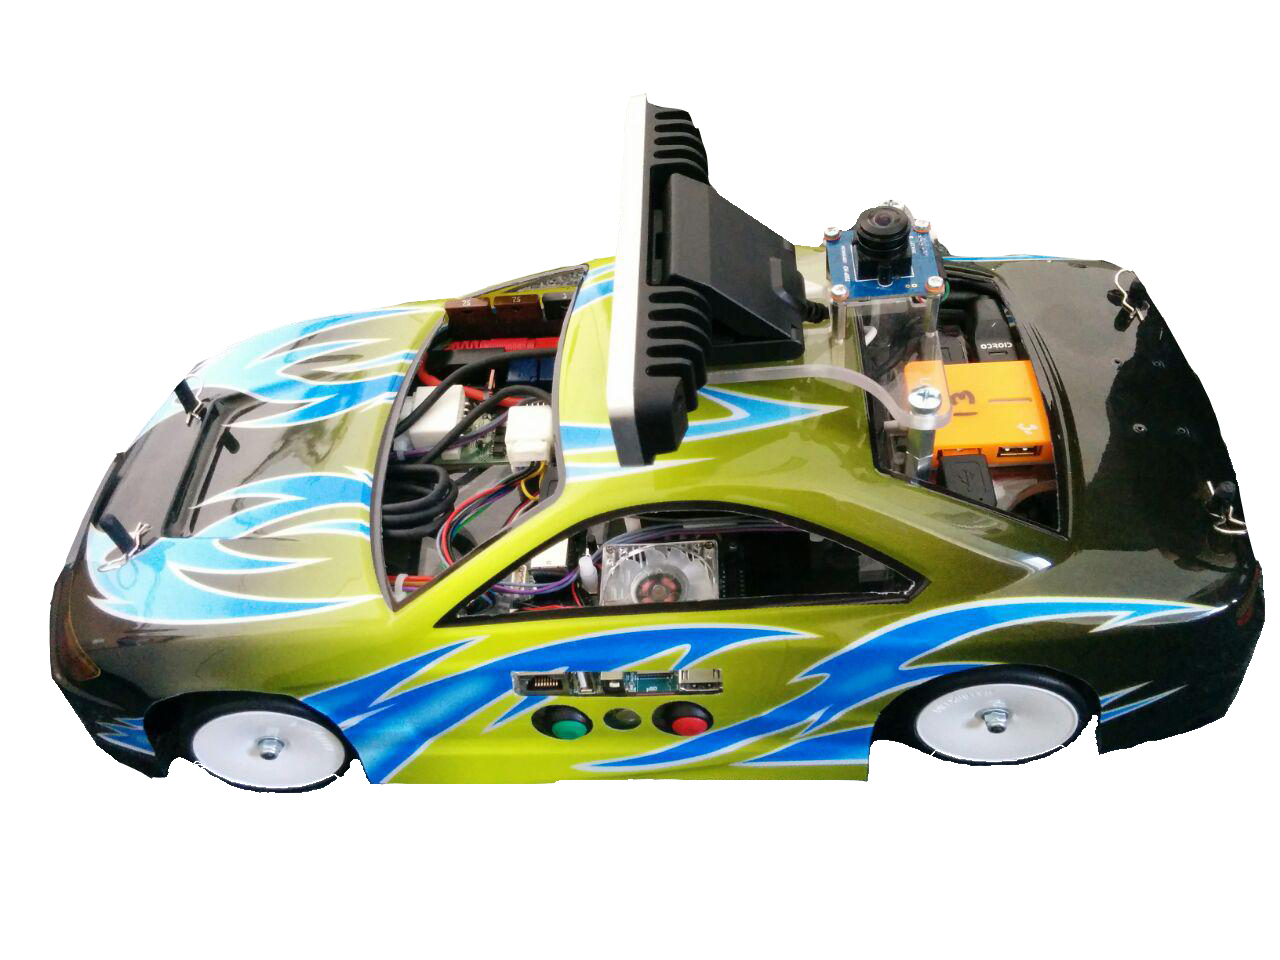
\includegraphics[width=0.8\textwidth]{Figures/coverpic.jpg}
  \caption{El vehículo AutoNOMOS}
\end{figure}
En ediciones anteriores no se permitían modificaciones de ningún tipo al hardware de estos vehículos, sin embargo, en esta edición del TMR se permitirá cualquier modificación siempre y cuando el vehículo resultante \textbf{no exceda los 65x25x20 cm (largo, ancho y alto)}.

\subsection{Plataformas abiertas}
Los vehículos de construcción propia deberán cumplir con las siguiente especificaciones:
\begin{itemize}
\item \textbf{El tamaño máximo deberá ser de 65 cm largo X 25 cm ancho X 20 cm alto.}
\item Se puede utilizar cualquier tipo de sensor, pero todos los dispositivos deben estar
montados en el robot.
\item Las demás restricciones descritas al inicio de esta sección.
\end{itemize}
Las dimensiones máximas se determinaron considerando que pueda participar un vehículo tipo camioneta pick-up a escala 1:10, aproximadamente. 

%%%%%%%%%%%%%%%%%%%%%%%%%%%%%%%%%%%%%%%
%%%%%%%%% SOBRE LA ARENA  %%%%%%%%%%%%%
%%%%%%%%%%%%%%%%%%%%%%%%%%%%%%%%%%%%%%%
\section{Sobre la arena}
\subsection{Pista de pruebas}
El desarrollo de las pruebas de conducción autónoma se realiza sobre una superficie de rodamiento consistente en una carpeta de material plástico artificial de 12 x 8 m, de color negro. Debe anticiparse cierto nivel de brillo o reflexión de la superficie de competencia. Sobre la
carpeta plástica se definen las líneas blancas correspondientes a los carriles que se muestra mediante impresión o cinta plastificada (de aislar). En la figura se muestra un ejemplo de circuito, con las especificaciones de anchos de carril, radios externos e internos de las curvas. El circuito que se use en la competencia podrá tener variaciones con respecto a esta descripción.

\begin{figure}
  \centering
  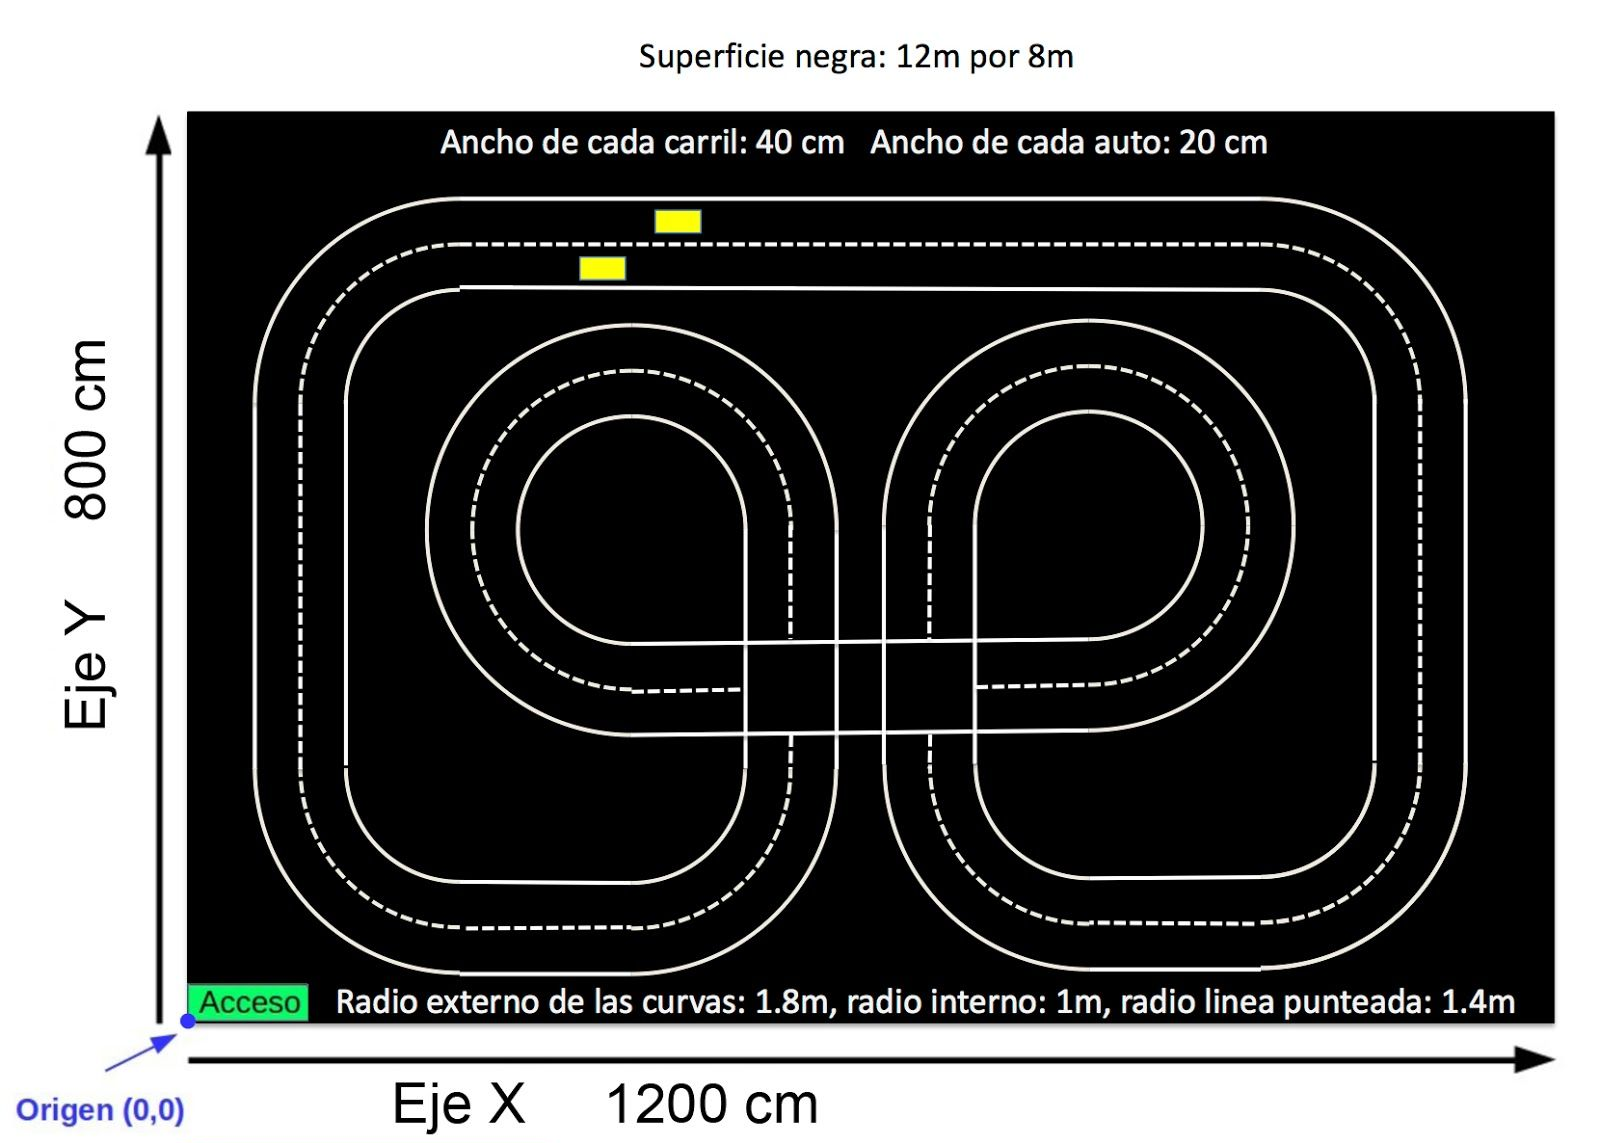
\includegraphics[width=\textwidth]{Figures/pista.png}
  \caption{Ejemplo de la pista de pruebas}
\end{figure}

En el ejemplo anterior, el circuito posee dos intersecciones en la parte central, donde los vehículos deberán ser capaces de detectar y evitar colisiones con otros vehículos que circulen por la pista (para las pruebas de navegación con obstáculos). 

\subsection{Zona de estacionamiento}
Asimismo, habrá una zona separada de la pista para las pruebas de estacionamiento lateral, como se ilustra en la figura. La banqueta será delimitada por “paredes” con altura suficiente para que pueda ser detectada por los sensores del robot. A diferencia de los años anteriores, el espacio para estacionarse estará delimitado por otros vehículos y no por paredes. Para este fin, se utilizarán los vehículos de otros equipos.
\begin{figure}
  \centering
  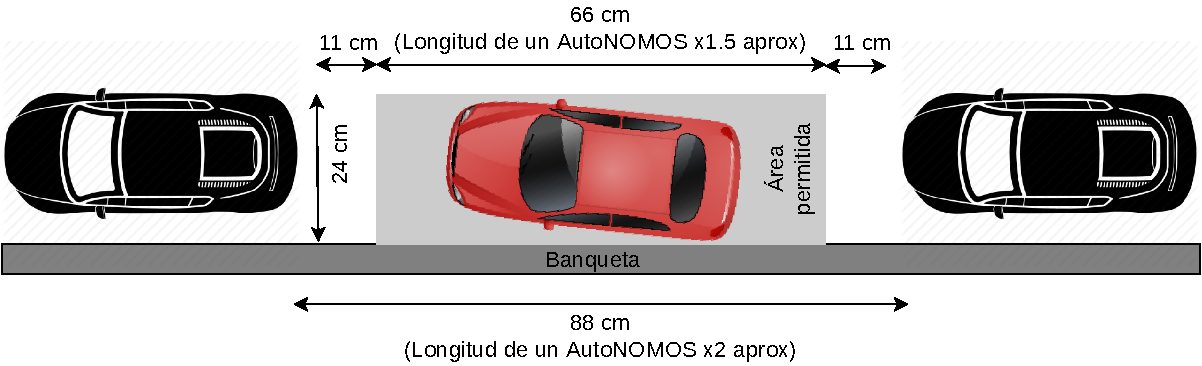
\includegraphics[width=0.8\textwidth]{Figures/Parking.pdf}
  \caption{Zona de estacionamiento}
  \label{fig:Parking}
\end{figure}

\subsection{Sobre la ambientación y objetos móviles}
Dependiendo del presupuesto disponible y/o patrocinios, eventualmente se podrá contar con ambientación dentro y/o alrededor de la pista de prueba, que simule objetos reales (edificios, comercios, árboles, etc.) que forman parte del entorno de navegación de un automóvil real. La intención a futuro es convertir la pista de pruebas en un modelo a escala 1:10 donde se incorporen paulatinamente las condiciones reales similares a las que un vehículo escala 1:1 se pudiese encontrar en su entorno normal de operación.

En cuanto a los obstáculos, se utilizarán los vehículos a escala de otros equipos, tanto para la prueba de navegación con obstáculos estáticos, como la prueba con obstáculos en movimiento.

%%%%%%%%%%%%%%%%%%%%%%%%%%%%%%%%%%%%%%%
%%%%%%%%%%%%% REGLAS %%%%%%%%%%%%%%%%%%
%%%%%%%%%%%%%%%%%%%%%%%%%%%%%%%%%%%%%%%
\section{Reglas}

Todas las pruebas se llevarán a cabo dentro de la pista bajo las siguientes reglas:

\textbf{1.} Bajo ninguna circunstancia se permitirá el control del automóvil por algún miembro de equipo. \textbf{La navegación debe ser autónoma} y la única ocasión en la que el equipo podrá intervenir es cuando se prepare el arranque inicial del vehículo o cuando se tenga que detener el mismo, ya sea debido a alguna colisión o por que el juez solicite un paro de emergencia.

\textbf{2.} El procesamiento deberá llevarse a cabo por completo a bordo del automóvil, sin embargo, para efectos de visualización y paro de emergencia será posible que el mismo envíe información sensorial o de estado a un equipo externo para su visualización, pero es importante
que el equipo muestre al juez que se cuenta con un mecanismo de paro con el cual detener al vehículo de manera inmediata en caso de requerirse. De no contar con ello, el equipo no podrá participar en prueba alguna. Por ningún motivo los integrantes del equipo deberán manipular la
aplicación de visualización durante la prueba, salvo en el caso de requerirse una acción de paro de emergencia.

\textbf{3.} Una vez que el automóvil arranque, ningún miembro del equipo participante podrá controlar al vehículo mediante joystick, dispositivo móvil o computadora. Un miembro del equipo participante deberá ser asignado como el ``piloto'' y por lo tanto sólo el podrá accionar los controles correspondientes para el arranque y el paro. El resto de los miembros deberá tener las manos libres a la vista del juez. De igual forma, el equipo de jueces podrá solicitar suscribirse a algún mecanismo de monitoreo de tópicos del automóvil del equipo, o incluso grabar
rosbags, o algún otro tipo de registro de datos . Ésto con la finalidad de verificar que no exista un control remoto del vehículo, pero también ayudaría a los equipos a recolectar datos en competencia que pudiesen utilizarse después para afinar los métodos implementados.

\textbf{4.} En la pista sólo se permitirá la presencia de un juez durante cualquiera de las pruebas. El juez tiene la autoridad para dar por terminada la prueba, en caso de que estime que el vehículo no cumpla con las reglas aquí estipuladas o que considere algún tipo de riesgo.

\textbf{5.} Las pruebas se ejecutarán una a la vez y sólo un equipo podrá ocupar la pista, a menos que se requiera la participación simultánea de otro equipo. Los demás equipos deberán esperar en la cola de participación y fuera de la arena en todo momento. Aquellas pruebas que impliquen la participación simultánea de más de un equipo se realizarán con la misma mecánica.

\textbf{6.} Se realizarán tres intentos por prueba. Para fines de monitoreo, sólo el equipo participante podrá tener encendida una red WiFi.

\textbf{7.} Los miembros del equipo podrán ingresar a la arena únicamente antes del inicio de la prueba, para colocar al automóvil o realizar ajustes (previamente autorizados por el juez), y posterior a que la prueba se ha dado por terminada. Sólo podrán ingresar aquellos miembros del equipo que cuenten con inscripción y lugar en mesa de trabajo, es decir, los mentores deberań permanecer fuera de la arena.

\textbf{8.} La pose inicial del automóvil (posición y dirección) será determinada por el comité técnico y podrá ser diferente para cada auto. Esta pose inicial se notificará al equipo en el momento de iniciar su prueba.

\textbf{9.} Si el automóvil participante choca contra algún objeto, persona, automóvil o ambientación dentro o fuera de la pista, la prueba se dará por terminada inmediatamente.

\textbf{10.} Si el automóvil pierde el control de manera abrupta, se impacta u ocasiona cualquier otro tipo de accidente, el equipo podrá quedar descalificado a criterio de los jueces, por ello es de vital importancia que el equipo participante siempre se encuentre alerta del estado del automóvil y que verifique que el mismo se pueda detener en cualquier momento.

\textbf{11.} Los equipos deberán llevar cargadas sus baterías al momento de ejecutar una prueba,esto es, no debe haber equipo de recarga de baterías al momento de efectuar la prueba y aquellas baterías cargadas que no se utilicen durante la misma deberán ser almacenadas en bolsas de seguridad de acuerdo al tipo de batería.

\textbf{12.} Queda estrictamente prohibido realizar pruebas fuera de la pista a excepción de aquellas realizadas por los equipos en sus mesas de trabajo y bajo su propia responsabilidad. Antes de la competencia se tendrán tiempos asignados para que los equipos realicen sesiones de
prueba, por lo que durante la competencia a excepción del equipo participante en turno, los equipos en la lista de espera para entrar a la arena no podrán encender cualquier tipo de aparato que pueda causar interferencia en las comunicaciónes del resto de autos que se encuentran
compitiendo dentro de la arena.
%%%%%%%%%%%%%%%%%%%%%%%%%%%%%%%%%%%%%%%
%%%%%%%%%%%%% PRUEBAS %%%%%%%%%%%%%%%%%
%%%%%%%%%%%%%%%%%%%%%%%%%%%%%%%%%%%%%%%
\section{Pruebas}
Existen cuatro pruebas en el mismo circuito que implican diferentes niveles de dificultad:

\begin{enumerate}
\item \textbf{Navegación Autónoma sin Obstáculos.} Consiste en cubrir el circuito de inicio a fin sin abandonar el carril correspondiente.
\item \textbf{Navegación Autónoma con Obstáculos.} Consiste en cubrir el circuito con tres obstáculos estáticos en la pista. Estos obstáculos serán los vehículos de otros equipos colocados aleatoriamente a lo largo del circuito.
\item \textbf{Navegación Autónoma con Obstáculos en Movimiento.} Consiste en cubrir el circuito con dos obstáculos estáticos y uno móvil. El vehículo del equipo participante deberá ejecutar una maniobra de rebase en esta prueba. El obstáculo se moverá a una velocidad suficientemente baja para que el vehículo participante pueda ejecutar el rebase. Los otros dos obstáculos estarán colocados aleatoriamente a lo largo del circuito.
  \item \textbf{Estacionamiento Autónomo.} Consiste en hacer que el vehículo pueda estacionarse en la zona designada (ver figura \ref{fig:Parking}). Se arrancará el vehículo a un metro de distancia, aproximadamente, del espacio para estacionarse. La posición y orientación inicial tendrán una ligera variación aleatoria para todos los equipos. 
\end{enumerate}

Cada equipo tendrá 10 minutos para ejecutar cada prueba (o repetir las que desee). Durante este tiempo, el equipo participante podrá solicitar máximo 2 reinicios, para lo cual no se detendrá el cronómetro. Si el equipo no se encuentra listo al momento de que le corresponda
efectuar la prueba, la misma se dará por concluida sin puntos y pierde su turno. En este caso el tiempo restante se dará como tiempo de preparación para que el resto de los equipos puedan hacer una prueba rápida, mientras le toca el turno al siguiente equipo en la lista. Los equipos en la cola de espera deben estar listos para participar inmediatamente en cuanto les toque su turno. El orden de participación se realizará en forma aleatoria al inicio del concurso y éste debe ser respetado. Cada equipo debe participar en el turno que le corresponde.

\subsection{Presentación del póster}
Consiste en presentar un póster con la descripción del equipo, características del hardware, descripción de los métodos utilizados y resultados obtenidos. El cartel deberá tener un tamaño A1 y deberá ser presentado en el lugar y hora que el comité organizador designe al principio de la competencia.\textbf{La presentación del póster no otorga puntos pero es obligatoria para la participación en las demás pruebas}.

%%%%%%%%%%%%%%%%%%%%%%%%%%%%%%%%%%%%%%%
%%%%%%%PUNTUACIÓN Y DESEMPATE %%%%%%%%%
%%%%%%%%%%%%%%%%%%%%%%%%%%%%%%%%%%%%%%%
\section{Sistema de puntuación y criterios de desempate}
Los principios para establecer la puntuación que un equipo alcanza serán simples:
\begin{itemize}
\item Quien concluye el circuito exitósamente en las pruebas 1, 2 y 3, obtiene mayor puntuación que quien no lo termina.
\item Los equipos que concluyen exitosamente una prueba se ordenarán de acuerdo al tiempo que requirieron para cubrir el circuito, en orden ascendente.
\item Se aplicarán penalizaciones en forma de un tiempo predefinido (ver sección \ref{sec:FinalScore} sobre las sanciones) que se deberá sumar al tiempo total requerido por el equipo para concluir la prueba. más las sanciones de tiempo recibidas.
\item El menor tiempo ganará la prueba.
\item Los equipos que no concluyen la prueba se ordenarán de acuerdo a la distancia del trayecto recorrido (durante un tiempo máximo de 5 minutos), restando 3 metros por cada minuto de sanciones acumulado. Por ejemplo, si alguien recorrió 9 metros en tres minutos y tiene un minuto de sanciones acumuladas se le asignará un recorrido total de 6 metros.
\item En la prueba sobre estacionamiento autónomo, se ordenará a los equipos de acuerdo al tiempo final requerido para concluir exitosamente la prueba, luego de aplicar sanciones a aquellos autos que colisionen contra algún obstáculo (ver sección \ref{sec:FinalScore}). Quien no logra estacionarse recibirá puntuación nula. Se considerará como exitosa la prueba si el vehículo queda estacionado dentro del espacio identificado en la Figura \ref{fig:Parking} como “Area permitida”.
\end{itemize}

%%%%%%%%%%%%%%%%%%%%%%%%%%%%%%%%%%%%%%%
%%%%%%%%%% CONTACTO %%%%%%%%%%%%%%%%%%%
%%%%%%%%%%%%%%%%%%%%%%%%%%%%%%%%%%%%%%%
\section{Contacto}

%%%%%%%%%%%%%%%%%%%%%%%%%%%%%%%%%%%%%%%
%%%%%%%%% CRÉDITOS %%%%%%%%%%%%%%%%%%%%
%%%%%%%%%%%%%%%%%%%%%%%%%%%%%%%%%%%%%%%
\section*{Créditos}
\end{document}

